\documentclass{article}

\usepackage{pandekten}
\usepackage{dashrule}

\makeatletter
\newcommand*{\shifttext}[1]{%
  \settowidth{\@tempdima}{#1}%
  \hspace{-\@tempdima}#1%
}
\newcommand{\plabel}[1]{%
\shifttext{\textbf{#1}\quad}%
}
\newcommand{\prule}{%
\begin{center}%
\hdashrule[0.5ex]{.99\linewidth}{1pt}{1pt 2.5pt}%
\end{center}%
}

\makeatother

\newcommand{\minusbaseline}{\abovedisplayskip=0pt\abovedisplayshortskip=0pt~\vspace*{-\baselineskip}}%

\setlength{\parindent}{0pt}

\title{Assignment 3}
\author{Ze Chen}

\begin{document}

\maketitle

\plabel{1}%
We anticipate oscillation of intensity as $\omega$ changes.

\plabel{(a)}%
The incidence electric field at $x_0 < x < 0$ is given by (dropping a global phase factor)
\[ \vb{E}_{\mathrm{i}}(x) = E_0 \hat{\vb{z}} \exp \qty(i k x), \]
where $k = \omega/c$ and
\[ E_0  = \frac{1}{2} c \mu_0 J_0. \]
With
\[ R = \frac{(n-1)^2}{(n+1)^2},\quad T = \frac{4n}{(n+1)^2}, \]
we find that the electric field at $2L$ is (with $\delta = 2nkL$)
\begin{align*}
    \vb{E}(2L) &= \frac{T e^{i\delta/2}}{1 - R e^{i\delta}} \times e^{ikL} \times \vb{E}_i(t,0) \\
    &= \frac{4n e^{inkL}}{(n+1)^2 - (n-1)^2 e^{2inkL}} \times e^{ikL} \times \frac{1}{2} c \mu_0 J_0 \hat{\vb{z}}.
\end{align*}
Inside the film, the right propagating part is given by
\begin{align*}
    \vb{E}_{\rightarrow}(x) = E_0 \hat{\vb{z}} \times \frac{t_{01}}{1 - R e^{i\delta}} e^{inkx}
\end{align*}
where
\[ t_{01} = \frac{2}{n+1}, \]
and the left propagating part is given by
\begin{align*}
    \vb{E}_{\leftarrow}(x) = E_0 \hat{\vb{z}} \times \frac{t_{01} r_{10} e^{i\delta}}{1 - R e^{i\delta}} e^{-inkx},
\end{align*}
where
\[ r_{10} = \frac{n-1}{n+1}. \]
The electric field in the film is
\begin{align*}
    \vb{E}(x) &= \vb{E}_{\rightarrow}(x) + \vb{E}_{\leftarrow}(x) \\
    &= E_0 \hat{\vb{z}} t_{10} \frac{(1-R r_{10}) \cos(n k x) + (r_{10} - R)\cos(n k x - \delta)}{1 + R^2 - 2 R \cos\delta}.
\end{align*}
Therefore,
\begin{align*}
    \abs{\vb{E}(x)}^2 &= \frac{E_0^2 t_{01}^2(1 + r_{10}^2 + 2r_{10} \cos(2knx - \delta))}{1+R^2 - 2R\cos\delta}, \\
    U(\omega) &= \frac{n^2}{4} \int_0^L \abs{\vb{E}}^2 \dd{x} \\
    &= \frac{E_0^2 n \left(2 k L n \left(n^2+1\right)+\left(n^2-1\right) \sin (2 k L n)\right)}{2 k \left(-\left(n^2-1\right)^2 \cos (2 k L n)+n^4+6 n^2+1\right)} \\
    &= \frac{E_0^2 n \left(2 (\omega/c) L n \left(n^2+1\right)+\left(n^2-1\right) \sin (2 (\omega/c) L n)\right)}{2 (\omega/c) \left(-\left(n^2-1\right)^2 \cos (2 \omega L n/c)+n^4+6 n^2+1\right)}.
\end{align*}

\plabel{(b)}%
For $U(\omega)$ we find
\begin{align*}
    A(\omega) &= \frac{E_0^2 \left(2 (\omega/c) L n \left(n^2+1\right)+\left(n^2-1\right) \sin (2 (\omega/c) L n)\right)}{16 n \omega / c} \\
    &= \frac{L E_0^2}{8} \qty[(n^2+1) + (n^2-1) \operatorname{sinc}\qty(\frac{2\pi\omega}{\Delta})] \\
    &= \frac{(c \mu_0 J_0)^2 L}{32}\qty[(n^2+1) + (n^2-1) \operatorname{sinc}\qty(\frac{2\pi \omega}{\Delta})], \\
    \mathcal{F} &= \frac{\pi(n^2-1)}{4n}, \\
    \Delta &= \frac{c\pi}{L n}.
\end{align*}
For
\[ \abs{\vb{E}(2L)}^2 = \frac{8 E_0^2 n^2}{1 + 6n^2 + n^4 - (n^2 - 1)^2 \cos(2 k L n)} \]
we find
\begin{align*}
    A(\omega) &= E_0^2 = \frac{(c \mu_0 J_0)^2}{4}, \\
    \mathcal{F} &= \frac{\pi(n^2-1)}{4n}, \\
    \Delta &= \frac{c\pi}{L n}.
\end{align*}

\plabel{(c)}%
The following is the plot of $U$.
\begin{center}
    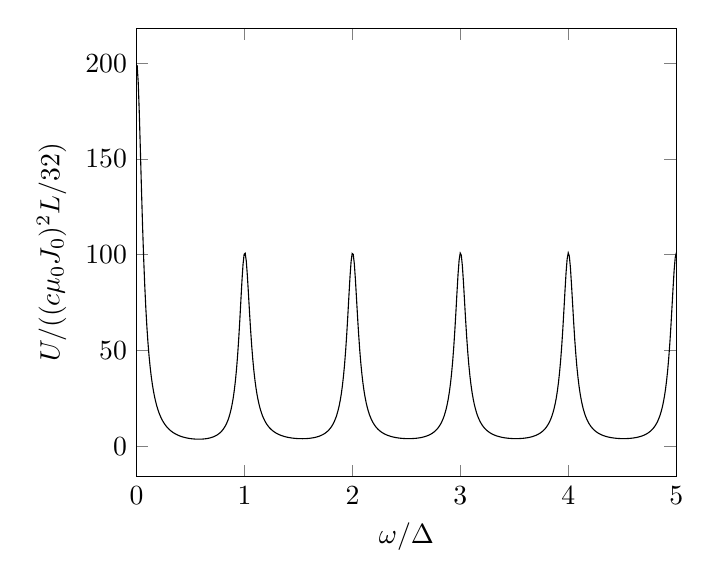
\begin{tikzpicture}
        \begin{axis}[xmin=0, xmax=5, samples=1000, xlabel=$\omega/\Delta$,ylabel=$U/((c\mu_0 J_0)^2L/32)$]
          \addplot[-] (x,{(101+99*sin(2*pi*x/pi*180)/(2*pi*x))/(1+(9801/400)*sin(pi*x/pi*180)^2)});
        \end{axis}
    \end{tikzpicture}
\end{center}
The following is the plot of $\abs{\vb{E}(2L)}^2$.
\begin{center}
    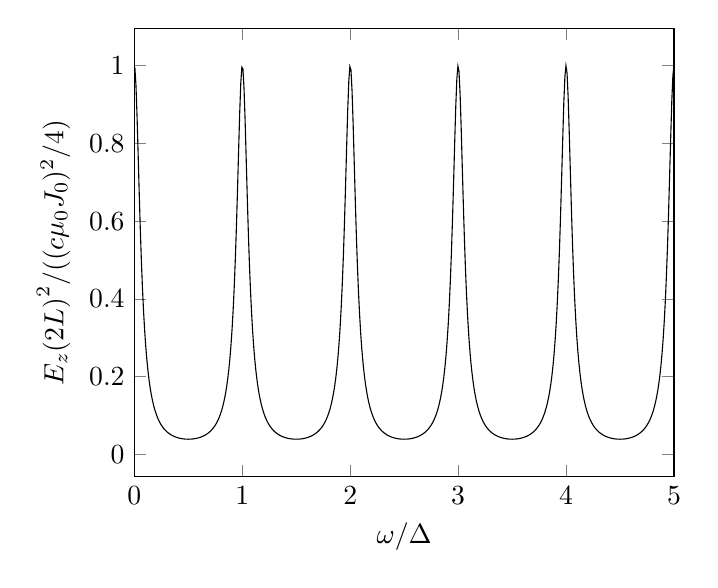
\begin{tikzpicture}
        \begin{axis}[xmin=0, xmax=5, samples=1000, xlabel=$\omega/\Delta$,ylabel=$\abs{E_z(2L)}^2/((c\mu_0 J_0)^2/4)$]
          \addplot[-] (x,{1/(1+(9801/400)*sin(pi*x/pi*180)^2)});
        \end{axis}
    \end{tikzpicture}
\end{center}
The scalings are indicated in the labels of axes.

\plabel{(d)}%
They both attain maxima when $\omega$ is a multiple of $\Delta$.
Higher $U$ implies higher constructive interference inside the film, and therefore the phases of waves are all equal at $x=L$.
This implies higher constructive interference on the right side of $x=L$, i.e. higher transmission.

\plabel{(e)}%
We plot for $\omega = \Delta$ and $\omega=1.5\Delta$.
\begin{center}
    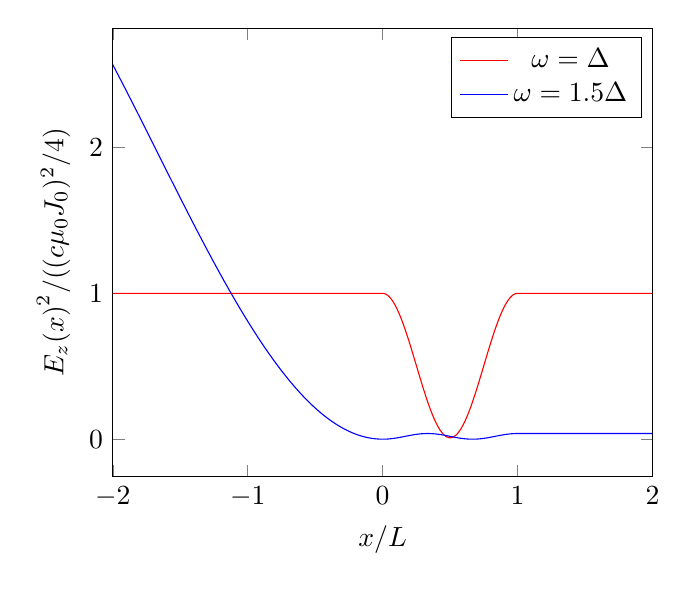
\begin{tikzpicture}
        \begin{axis}[xmin=-2, xmax=2, samples=1000, xlabel=$x/L$,ylabel=$\abs{E_z(x)}^2/((c\mu_0 J_0)^2/4)$]
          \addplot[-,red] {x > 1 ? 1 : (x > 0 ? (1/200*(101+99*cos(2*pi*x/pi*180))) : 1)};
          \addplot[-,blue] {x > 1 ? (400/10201) : (x > 0 ? (2/10201*(101-99*cos(3*pi*x/pi*180))) : (2*(10001-9999*cos(3*pi*x/10/pi*180))/10201))};
          \legend{$\omega=\Delta$,$\omega=1.5\Delta$}
        \end{axis}
    \end{tikzpicture}
\end{center}

\prule
\plabel{2 (a)}%
The $S$ matrix of the mirror at input and output is
\[ S = \begin{pmatrix}
    -r_0 & it_0 \\
    it_0 & -r_0
\end{pmatrix}. \]
Tracing the beams we find
\[ \begin{pmatrix}
    b_2 \\ b_1
\end{pmatrix} = e^{i k_0 n_0 (L_1+L_2+L_3)} S^2 \begin{pmatrix}
    a_1 \\ 0
\end{pmatrix} = e^{i k_0 n_0 (L_1+L_2+L_3)} \begin{pmatrix}
    r_0^2 - t_0^2 \\
    -2 i r_0 t_0
\end{pmatrix} a_1. \]
The power transmissions are given by
\begin{align}
    \label{eq:e2}\frac{\abs{b_2}^2}{\abs{a_1}^2} &= (r_0^2 - t_0^2)^2, \\
    \label{eq:e1}\frac{\abs{b_1}^2}{\abs{a_1}^2} &= 4r_0^2 t_0^2.
\end{align}
It's clear that, since $(r_0^2 - t_0^2)^2 + \abs{-2ir_0t_0}^2 = (r_0^2 + t_0^2)^2 = 1$,
\[ \frac{\abs{b_2}^2}{\abs{a_1}^2} + \frac{\abs{b_1}^2}{\abs{a_1}^2} = 1. \]

\plabel{(b)}%
%Denote by $c_{ij}$ the field at the mirror going from $L_i$ to $L_j$.
Let the $S_Q$ be the $S$ matrix of $Q$, i.e.
\[ S_Q = \frac{1}{1- r^2 e^{i\delta}} \begin{pmatrix}
    r(1-e^{i\delta}) & T e^{i\delta/2} \\
    T e^{i\delta/2} & r(1-e^{i\delta})
\end{pmatrix}, \]
where $T = 1-r^2$, $r = (n_1 - n_0)/(n_1 + n_0)$, and
\[ \delta = 2 k_0 n_1 L_Q. \]
We have
\begin{align*}
    \begin{pmatrix}
        b_2 \\ b_1
    \end{pmatrix} = e^{ik_0n_0(L_1+L_2+L_3-L_Q)} S S_Q S \begin{pmatrix}
        0 \\ a_1
    \end{pmatrix}.
\end{align*}
We find
\begin{align*}
    b_2 &= e^{ik_0n_0(L_1+L_2+L_3-L_Q)}  \frac{ e^{\frac{i \delta }{2}} \left(1-r^2\right) (r_0^2-t_0^2)  - 2 i (1-e^{i\delta})r r_0 t_0 }{1- r^2 e^{i \delta }} a_0, \\
    b_1 &= e^{ik_0n_0(L_1+L_2+L_3-L_Q)}   \frac{-2 i e^{\frac{i \delta }{2}} \left(1-r^2\right) r_0 t_0 + (1 - e^{i \delta }) r (r_0^2-t_0^2)}{1-e^{i \delta } r^2} a_0.
\end{align*}
The power transmissions are given by
\begin{align*}
    \frac{\abs{b_2}^2}{\abs{a_1}^2} &= \frac{\left(\left(1-r^2\right) (r_0^2 - t_0^2) - 4 r r_0 t_0 \sin \left(\delta/2\right)\right)^2}{1 -2 r^2 \cos \delta +r^4}, \\
    \frac{\abs{b_1}^2}{\abs{a_1}^2} &= \frac{4 \left(\left(r^2-1\right) r_0 t_0 +r \sin \left(\delta/2\right) \left(r_0^2 - t_0^2\right)\right)^2}{1-2 r^2 \cos \delta +r^4}.
\end{align*}

Setting $r = 0$ we retrieve the result in \cref{eq:e2,eq:e1}.
In such case, the existence of $Q$ may be detected by an interferometer.

\plabel{(c)}%
Let $I = \alpha \abs{a}^2$ where $I$ is the strength, i.e. we absorb all constant factors into $\alpha$.
Then $\phi_{\mathrm{NL}} = k_0 n_2 \alpha \abs{a}^2 L_Q$ where $a$ is the field strength of the incidence beam.
We work in the case where $r=0$, i.e. $Q$ does not reflect.
Although $S_Q$ is no longer linear, we may abuse the notation and write
\[ S_Q = \begin{pmatrix}
    & e^{i k_0 n_2 L_Q} \exp(i k_0 n_2 L_Q \alpha \abs{\bullet}^2) \\
    e^{i k_0 n_2 L_Q} \exp(i k_0 n_2 L_Q \alpha \abs{\bullet}^2)
\end{pmatrix}. \]
Again from 
\begin{align*}
    \begin{pmatrix}
        b_2 \\ b_1
    \end{pmatrix} = e^{ik_0n_0(L_1+L_2+L_3-L_Q)} S S_Q S \begin{pmatrix}
        0 \\ a_1
    \end{pmatrix}.
\end{align*}
we find
\begin{align*}
    \begin{pmatrix}
        b_2 \\ b_1
    \end{pmatrix} &= e^{ik_0n_0(L_1+L_2+L_3-L_Q) + ik_0n_1L_Q} a_1 \times \\
    &\phantom{{}={}} \begin{pmatrix}
        r_0^2 \exp(i k_0 n_2 L_Q r_0^2 \alpha \abs{a_1}^2) - t_0^2 \exp(i k_0 n_2 L_Q t_0^2 \alpha \abs{a_1}^2) \\
        -i r_0 t_0 \qty(\exp(i k_0 n_2 L_Q r_0^2 \alpha \abs{a_1}^2) + \exp(i k_0 n_2 L_Q t_0^2 \alpha \abs{a_1}^2))
    \end{pmatrix}.
\end{align*}
Therefore,
\begin{align*}
    \frac{\abs{b_2}^2}{\abs{a_1}^2} &= r_0^4+t_0^4-2 r_0^2 t_0^2 \cos \left(\alpha \abs{a_1}^2 k_0 n_2 L_Q (r_0^2 - t_0^2)\right), \\
    \frac{\abs{b_1}^2}{\abs{a_1}^2} &= 2 r_0^2 t_0^2 \left(1+\cos \left(\alpha \abs{a_1}^2 k_0 n_2 L_Q (r_0^2 - t_0^2)\right)\right).
\end{align*}
The transmissions are increased (or decreased) by 
\[ 2 r_0^2 t_0^2 \cos \left(\alpha \abs{a_1}^2 k_0 n_2 L_Q (r_0^2 - t_0^2)\right). \]

\plabel{(d)}%
Transmissions attain extrema if the phase factor in $\cos(\cdots)$ is a multiple of $\pi$, i.e.
\[ \abs{a_1}^2 = \frac{m \pi}{\alpha k_0 n_2 L_Q (r_0^2 - t_0^2)} \]
for some integer $m$.

\plabel{(e)}%
In the nonlinear case the wave equation is given by
\[ \Box^2 \vb{E} \sim \vb{E}\vb{E}. \]
When there are two waves in the medium, the equation for each wave becomes
\[ \Box^2 \vb{E}_1 \sim (\vb{E}_1 + \vb{E}_2) \vb{E}_1. \]
The first term gives rise to the self-phase shift while the second term gives rise to the cross-phase modulation.

% \bibliographystyle{plain}
% \bibliography{main}

\end{document}
